\section{PySide}

\begin{figure}[h]
\centering 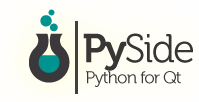
\includegraphics[scale=0.7]{images/Pyside.png}
\caption{Python logo}
\end{figure}

\subsection{Introduction}
PySide is an open source software project providing Python bindings for the Qt framework. Qt is a cross-platform application and UI framework, allowing the developers to write applications once and deploy them across many operating systems without rewriting the source code, while Python is a modern, dynamic programming language with a vivid developer community.

Combining the power of Qt and Python, PySide provides the wealth of Qt framework for developers writing software in Python and presents a first-class rapid application development platform available on all major operating systems.

\subsection{Licensing}
PySide has been published as a response to the lack of suitably licensed Qt bindings for Python. PySide is licensed under the LGPL version 2.1 license, allowing both Free/Open source software and proprietary software development.

\subsection{Project scope and goals}
PySide consists of a full set of Qt and Qt Quick bindings for multiple platforms as well as the automated binding generation tools required to produce the bindings. Due to the availability of the whole toolchain, PySide will be of interest not only to developers requiring the Qt bindings, but to developers willing to generate other Qt and C++ based bindings as well.

Although based on a different technology than the competing PyQt bindings, in the Python-level compatibility between the two projects is still rather high, allowing for easy porting of software between PyQt and PySide.

The PySide project has been initiated and much of the initial development sponsored by Nokia. PySide is now run as a true open source project, and currently most of new work is based on volunteer contributor efforts. PySide is a Qt add-on, utilizing the same licensing and the same infrastructure as Qt itself.

PySide aims to support all the platforms Qt itself does. Feel welcome to assist in porting the code to your platform of choice.

\subsection{Installation of PySide}
To install PySide, you can choose from the following options:
\begin{itemize}
\item Use pip to install the wheel binary packages:
\begin{verbatim}
pip install -U PySide
\end{verbatim}

\item Use setuptools to install the egg binary packages (deprecated):
\begin{verbatim}
easy_install -U PySide
\end{verbatim}

\end{itemize}

\subsection{Hello World example}
\begin{verbatim}
# Import PySide classes
import sys
from PySide.QtCore import *
from PySide.QtGui import *

# Create a Qt application
app = QApplication(sys.argv)

# Create a Window
mywindow = QWidget()
mywindow.resize(320, 240)
mywindow.setWindowTitle('Hello World!')

# Create a label and display it all together
mylabel = QLabel(mywindow)
mylabel.setText('Hello World!')
mylabel.setGeometry(QRect(130, 110, 60, 10))
mywindow.show()

# Enter Qt application main loop
sys.exit(app.exec_())
\end{verbatim}


